\PassOptionsToPackage{unicode=true}{hyperref} % options for packages loaded elsewhere
\PassOptionsToPackage{hyphens}{url}
%
\documentclass[doc]{apa6}
\usepackage{lmodern}
\usepackage{amssymb,amsmath}
\usepackage{ifxetex,ifluatex}
\usepackage{fixltx2e} % provides \textsubscript
\ifnum 0\ifxetex 1\fi\ifluatex 1\fi=0 % if pdftex
  \usepackage[T1]{fontenc}
  \usepackage[utf8]{inputenc}
  \usepackage{textcomp} % provides euro and other symbols
\else % if luatex or xelatex
  \usepackage{unicode-math}
  \defaultfontfeatures{Ligatures=TeX,Scale=MatchLowercase}
\fi
% use upquote if available, for straight quotes in verbatim environments
\IfFileExists{upquote.sty}{\usepackage{upquote}}{}
% use microtype if available
\IfFileExists{microtype.sty}{%
\usepackage[]{microtype}
\UseMicrotypeSet[protrusion]{basicmath} % disable protrusion for tt fonts
}{}
\IfFileExists{parskip.sty}{%
\usepackage{parskip}
}{% else
\setlength{\parindent}{0pt}
\setlength{\parskip}{6pt plus 2pt minus 1pt}
}
\usepackage{hyperref}
\hypersetup{
            pdftitle={Sans Forgetica is Really Forgettable?},
            pdfauthor={Jason Geller, Sara D. Davis, \& Daniel Peterson},
            pdfkeywords={fluency},
            pdfborder={0 0 0},
            breaklinks=true}
\urlstyle{same}  % don't use monospace font for urls
\usepackage{graphicx,grffile}
\makeatletter
\def\maxwidth{\ifdim\Gin@nat@width>\linewidth\linewidth\else\Gin@nat@width\fi}
\def\maxheight{\ifdim\Gin@nat@height>\textheight\textheight\else\Gin@nat@height\fi}
\makeatother
% Scale images if necessary, so that they will not overflow the page
% margins by default, and it is still possible to overwrite the defaults
% using explicit options in \includegraphics[width, height, ...]{}
\setkeys{Gin}{width=\maxwidth,height=\maxheight,keepaspectratio}
\setlength{\emergencystretch}{3em}  % prevent overfull lines
\providecommand{\tightlist}{%
  \setlength{\itemsep}{0pt}\setlength{\parskip}{0pt}}
\setcounter{secnumdepth}{0}
% Redefines (sub)paragraphs to behave more like sections
\ifx\paragraph\undefined\else
\let\oldparagraph\paragraph
\renewcommand{\paragraph}[1]{\oldparagraph{#1}\mbox{}}
\fi
\ifx\subparagraph\undefined\else
\let\oldsubparagraph\subparagraph
\renewcommand{\subparagraph}[1]{\oldsubparagraph{#1}\mbox{}}
\fi

% set default figure placement to htbp
\makeatletter
\def\fps@figure{htbp}
\makeatother

\shorttitle{Sans Forgetica}
\affiliation{
\vspace{0.5cm}
\textsuperscript{1} University of Iowa\\\textsuperscript{2} Skidmore College}
\keywords{fluency\newline\indent Word count: X}
\usepackage{csquotes}
\usepackage{upgreek}
\captionsetup{font=singlespacing,justification=justified}

\usepackage{longtable}
\usepackage{lscape}
\usepackage{multirow}
\usepackage{tabularx}
\usepackage[flushleft]{threeparttable}
\usepackage{threeparttablex}

\newenvironment{lltable}{\begin{landscape}\begin{center}\begin{ThreePartTable}}{\end{ThreePartTable}\end{center}\end{landscape}}

\makeatletter
\newcommand\LastLTentrywidth{1em}
\newlength\longtablewidth
\setlength{\longtablewidth}{1in}
\newcommand{\getlongtablewidth}{\begingroup \ifcsname LT@\roman{LT@tables}\endcsname \global\longtablewidth=0pt \renewcommand{\LT@entry}[2]{\global\advance\longtablewidth by ##2\relax\gdef\LastLTentrywidth{##2}}\@nameuse{LT@\roman{LT@tables}} \fi \endgroup}


\usepackage{lineno}

\linenumbers

\title{Sans Forgetica is Really Forgettable?}
\author{Jason Geller\textsuperscript{1}, Sara D. Davis\textsuperscript{2}, \& Daniel Peterson\textsuperscript{2}}
\date{}

\authornote{Add complete departmental affiliations for each author here. Each new line herein must be indented, like this line.

Enter author note here.

Correspondence concerning this article should be addressed to Jason Geller, Postal address. E-mail: \href{mailto:jason-geller@uiowa.edu}{\nolinkurl{jason-geller@uiowa.edu}}}

\abstract{

}

\begin{document}
\maketitle

Students want to remember more and forget less. Decades of research have put forth the paradoxical idea that making learning harder (not easier) should have the desirable effect of improving long-term retention of material--called the desirable diffuclty principle (Bjork, 1994). Notable examples of desirable difficulties include having participants generate information from word fragments instead of passively reading intact words (e.g., Slamecka \& Graf, 1978), spacing out study sessions instead of massing them (e.g., Carpenter, 2017), and having participants engage in retrieval practice after studying instead of simply restudying the information (Kornell \& Vaughn, 2016). Another simple strategy that has gained some attention is to make material more perceptually disfluent. This can be done by changing the material's perceptual characteristics (Diemand-Yaumen, Oppenheimer, \& Vaughan, 2011; French et al., 2013). Visual material that is masked (Mulligan, 1996), inverted (Sungkhasette, Friedman, \& Castel, 2011), presented in an atypical font (Diemand Yaumen et al., 2011), blurred (Rosner, Davis, \& Milliken, 2015), or even in handwritten cursive (Geller, Still, Dark, Carpenter, 2018) have all been shown to produce memory benefits. The desirable effect of perceptual disfluency on memory is called called the disfluency effect.

Although appealing as a pedagogical strategy, there have been several experiments that failed to find memorial benefits for perceptually disfluent
materials (e.g., Magreehan, Serra, Schwartz \& Narciss, 2016; Rhodes \& Castel, 2008, 2009; Rummer, Scheweppe, \& Schewede, 2016; Yue,
Castel, \& Bjork, 2013), casting doubt upon the veracity of the disfluency effect. A recent meta-analysis (), Recent studies by Geller et al.(2018) and Geller \& Still (2018) found that perceptual disfluency can have a beneficial effect on memory, but seems to be rather fickle, thus delimiting its educational usefuleness.

Given the weak evidence, it came as a surprise to me when a little over a year ago, a font by the name of Sans Forgetica (SF) started getting a ton of press coverage. The mnnmenomic benefits of this font, \emph{based on cognitive psychology}, were being touted in reputable news sources like Washington Post (\url{https://www.washingtonpost.com/business/2018/10/05/introducing-sans-forgetica-font-designed-boost-your-memory/}) and NPR (\url{https://www.npr.org/2018/10/06/655121384/sans-forgetica-a-font-to-remember}, amongst others. The creators even made the SF font available for mac and pc operating systems--all you have to do is downlaod the font file and you to can remember everything you read :). There is even a Chrome browser extension and cellphone application that allows users to place material in Sans Forgetica. With this much attention and marketing, there has to be solid empirical evidence backing it up, right? Not quite.

Despite the weak evidence for perceptual disfluency, it came as a surprise to me when a little over a year ago, I saw a font by the name of Sans Forgetica (SF) getting a ton of press coverage. The mnnmenomic benefits of this font, \emph{based on cognitive psychology}, were being touted in reputable news sources like Washington Post (\url{https://www.washingtonpost.com/business/2018/10/05/introducing-sans-forgetica-font-designed-boost-your-memory/}) and NPR (\url{https://www.npr.org/2018/10/06/655121384/sans-forgetica-a-font-to-remember}, amongst others. The creators even made the SF font available for mac and pc operating systems--all you have to do is downlaod the font file and you to can remember everything you read :). There is even a Chrome browser extension and cellphone application that allows users to place material in Sans Forgetica. With this much attention and marketing, there has to be solid empirical evidence backing it up, right? Not quite.

\hypertarget{what-do-we-know-about-sf}{%
\section{What do we know about SF?}\label{what-do-we-know-about-sf}}

There is not information about SF. The typyface itself is a variation of a sans-serif typeface. It is a typeface that consists of intermitten gaps in letters that are back slanted (see below picture). The design features of this typeface require readers of it to \enquote{fill-in} the missing pieces like a puzzle. As it pertains to the empirical validation of the claims made, the website does offer some information about SF and how the original results were obtained, but not enough information to replicate the studies.

\begin{figure}
\centering
\includegraphics{https://user-images.githubusercontent.com/18429968/70854186-006bd180-1e7e-11ea-8fe1-94f5cf37c805.png}
\caption{image}
\end{figure}

\hypertarget{earp-2018-conducted-an-interview-with-the-creators-of-sf-and-here-is-what-we-know.-apparently-two-studies-were-conducted.-in-a-lab-experiment-n96-they-had-participants-read-20-word-pairs-e.g.-girl---guy-called-a-paried-associates-task-in-cognitive-parlance-in-three-new-fonts-one-of-them-being-sf-and-a-typical-or-common-font.-the-font-pairs-were-presented-were-counterbalanced-across-participants.-what-this-means-is-that-all-fonts-were-shown-but-the-same-pairs-were-never-presneted-in-more-than-one-type-of-font.-each-word-pair-was-presnted-on-the-screen-for-100-ms-that-is-super-fast.-for-a-final-test-they-were-given-the-cue-e.g.-girl-and-had-to-respond-with-the-target-guy.-what-did-they-find-according-to-the-interview-targets-were-recalled-68-of-time-when-presented-in-a-common-font.-for-cue-target-pairs-in-sf-targets-were-recalled-69-of-the-timea-negeliable-difference.}{%
\section{\texorpdfstring{Earp (2018) conducted an interview with the creators of SF and here is what we know. Apparently two studies were conducted. In a lab experiment (\emph{N}=96), they had participants read 20 word pairs (e.g., girl - guy; called a paried associates task in cognitive parlance) in three new fonts (one of them being SF) and a typical or common font. The font pairs were presented were counterbalanced across participants. What this means is that all fonts were shown, but the same pairs were never presneted in more than one type of font. Each word pair was presnted on the screen for 100 ms (that is super fast\ldots{}). For a final test, they were given the cue (e.g., \emph{girl}) and had to respond with the target (\emph{guy}). What did they find? According to the interview, targets were recalled 68\% of time when presented in a common font. For cue-target pairs in SF, targets were recalled 69\% of the time--a negeliable difference.}{Earp (2018) conducted an interview with the creators of SF and here is what we know. Apparently two studies were conducted. In a lab experiment (N=96), they had participants read 20 word pairs (e.g., girl - guy; called a paried associates task in cognitive parlance) in three new fonts (one of them being SF) and a typical or common font. The font pairs were presented were counterbalanced across participants. What this means is that all fonts were shown, but the same pairs were never presneted in more than one type of font. Each word pair was presnted on the screen for 100 ms (that is super fast\ldots{}). For a final test, they were given the cue (e.g., girl) and had to respond with the target (guy). What did they find? According to the interview, targets were recalled 68\% of time when presented in a common font. For cue-target pairs in SF, targets were recalled 69\% of the time--a negeliable difference.}}\label{earp-2018-conducted-an-interview-with-the-creators-of-sf-and-here-is-what-we-know.-apparently-two-studies-were-conducted.-in-a-lab-experiment-n96-they-had-participants-read-20-word-pairs-e.g.-girl---guy-called-a-paried-associates-task-in-cognitive-parlance-in-three-new-fonts-one-of-them-being-sf-and-a-typical-or-common-font.-the-font-pairs-were-presented-were-counterbalanced-across-participants.-what-this-means-is-that-all-fonts-were-shown-but-the-same-pairs-were-never-presneted-in-more-than-one-type-of-font.-each-word-pair-was-presnted-on-the-screen-for-100-ms-that-is-super-fast.-for-a-final-test-they-were-given-the-cue-e.g.-girl-and-had-to-respond-with-the-target-guy.-what-did-they-find-according-to-the-interview-targets-were-recalled-68-of-time-when-presented-in-a-common-font.-for-cue-target-pairs-in-sf-targets-were-recalled-69-of-the-timea-negeliable-difference.}}

Earp (2018) conducted an interview with the creators of SF and I was able to glean some details about how SF ws validated. Apparently two studies were conducted. In a lab experiment (\emph{N}=96), they had participants read 20 word pairs (e.g., girl - guy; called a paried associates task in cognitive parlance) in three new fonts (one of them being SF) and a typical or common font. The font pairs were presented in was counterbalanced participants. What this means is that all fonts were showns, but the same pairs were never presneted in more than one type of font. Each word pair was presnted on the screen for 100 ms (that is super fast\ldots{}). For a final test, they were given the cue (e.g., \emph{girl}) and had to respond with the target (\emph{guy}). What did they find? According to the interview, targets were recalled 68\% of time when presented in a common font. For cue-target pairs in SF, targets were recalled 69\% of the time--a negeliable difference.

In an online experiment, participants were presented passages (250 words in total) where one of the paragraphs was presented in SF. Each participant saw five different texts in total. For each text they were asked one question about the part written in SF and another question about the part written in standard Arial. Participants remembered 57\% of the text when a section was written in Sans Forgetica, compared to 50\% of the surrounding text that was written in a plain Arial font.

At the time of this writing, these studies have not been published nor is there a preprint available. I reached out to the creators of SF, but they refused to share the materials with me. Instead of waiting, I elicited the help of Sara Davis and Daniel Peterson at Skidmore university to test the mnenmomic benefits of Sans Forgetica. We preregistered two studies (\url{https://osf.io/d2vy8/}). All materials, data, and analysis scripts can be found at that website. Analyses are computationally reproducible by going to this github and clicking on the binder button. the two reported experiments in an online container (\url{https://github.com/jgeller112/SF_Expt1}; \url{https://github.com/jgeller112/SF_Expt2}).

\hypertarget{experiment-1}{%
\section{Experiment 1}\label{experiment-1}}

In the first study we compared the mnenmonic benefits of SF against a robust technique known to enhance memory---generation. The generation effect is a phenomenon where information is better remembered when retrieved than if it is simply read. In a prototypical experiment,participants are asked to generate words from word fragments DOLL - DR\_\_ or read intact cue-target pairs (\emph{DOLL-DRESS}). Compared to the intact condition, individuals recall the generated target words at a higher rate. The nature of generation is where the supposed mnnmeoic benefit of SF comes from. We examined this in the current experiment.

\hypertarget{participants}{%
\subsection{Participants}\label{participants}}

We recruited 230 people from Amazon's Mechanical Turk Service. Sample size was calculated based on the smallest effect of interest (SEOI; Lakens \& Evers, 2014). In this case, we were interested in powering our study to detect a medium-sized effect size (\emph{d} = .35). We choose this effect size as our SESOI due in part to the small effect sizes seen in actaul classroom studies (Bulter et al., 2014). Therefore, assuming an alpha of .05 and a desired power of 90\%, a sample size of 270 is required to detect whether an effect size of .35 differs from zero. After excluding participants After excluding participants who 1) did not complete every phase of the experiment, 2) started the experiment multiple times, 3) reported experiencing technical problems did not indicate that they were fluent in English {[}\^{}2{]}: This question was not asked during the experiment., or 5) reported seeing our stimuli before we were left with 115 participants per group.

\hypertarget{materials-and-procedure}{%
\subsection{Materials and Procedure}\label{materials-and-procedure}}

all

Participants were presented with 22 weakly related cue-target pairs taken from Carpenter et al., 2012){[}\^{}1{]}: Two cue-target pairs () had to be thrown out as they were not preseted due to a coding error. The cue-target pairs were all nouns, 5--7 letters and 1--3 syllables in length, and high in concreteness (400--700) and frequency (at least 30 per million).

For half the participants, targets were presented in SF while the other half were presented in Arial font; for the other half of participants, targets were presented with missing letters (vowels were replaced by underscores) and the other half were intact (Arial font). After a short 2 minute distractor task (anagram generation), they completed a cued recall test. During cued recall, particpants were presented 24 cues one at a time and asked to provide the target word. After they were thanked and debriefed.

In Experiment 1 participants were presented with 40 weakly relatedcue-target pairs. The pairs were nouns, 5--7 letters, 1--3 syllables in length, and high in concreteness (400--700) and frequency (at least 30 per million). For half of the participants, half of the targets were presented in SF while the other half were presented in Arial font; for the other half of participants, the targets were presented with missing letters (vowels were replaced by underscores) and the other half were intact (Arial font). After a short 2 minute distractor task (anagram generation), they completed a cued recall test.

Spell checking was automated with the hunspell package in R (Ooms, 2018) using spellCheck.R. Becasuse participants were recruited in the United States, we used the American English dictionary. A nice walkthrough on how to use the package can be found in Buchcamam, De Deyne, \& Montefinese (2019). Using the package, each response was corrected for misspelings. Corrected spellings are provided in the most probable order, therefore, the first suggestion is selected as the correct answer. Answers were marked correct if they provided the exact response. In order for a response to be judged correctly, the response had to match the correct answer.

What did we find?

In Experiment 1 we found a sizeable generation effect, which replicated past work. However, we did not find a SF effect (See figure below)

\begin{verbatim}
## Warning: Missing column names filled in: 'X1' [1]
\end{verbatim}

\begin{verbatim}
## 
##  condition*dis effect
##                 dis
## condition        disfluent    fluent
##   Generate       0.2952348 0.1507106
##   Sans Forgetica 0.2429061 0.2469149
## 
##  Lower 95 Percent Confidence Limits
##                 dis
## condition        disfluent     fluent
##   Generate       0.1625725 0.08088777
##   Sans Forgetica 0.1343397 0.14399034
## 
##  Upper 95 Percent Confidence Limits
##                 dis
## condition        disfluent    fluent
##   Generate       0.4747772 0.2635241
##   Sans Forgetica 0.3987912 0.3898998
\end{verbatim}

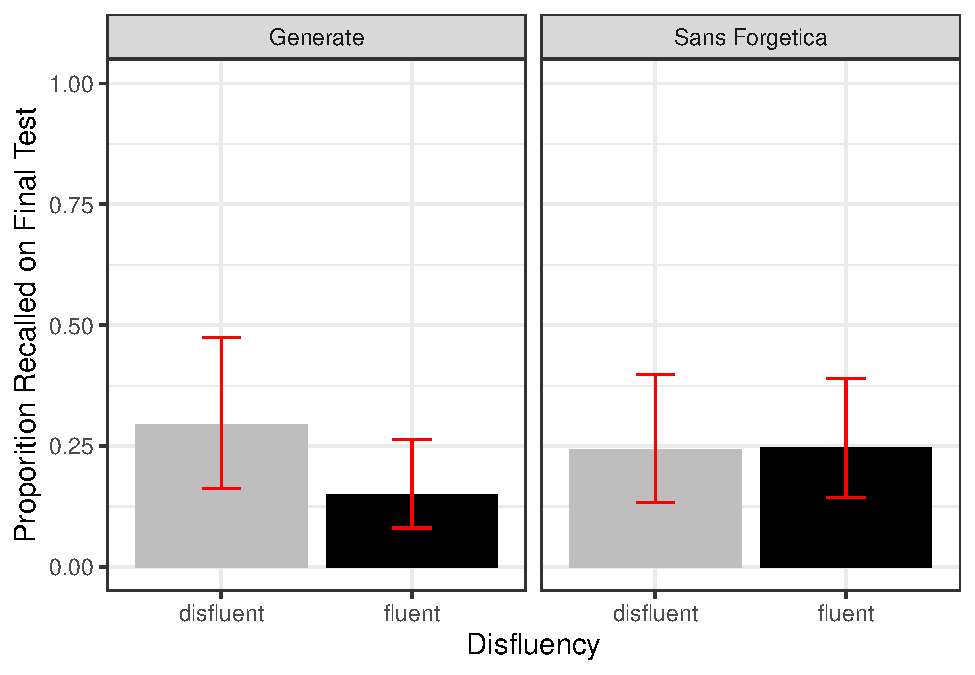
\includegraphics{SF_Paper_files/figure-latex/unnamed-chunk-1-1.pdf}

\hypertarget{experiment-2}{%
\section{Experiment 2}\label{experiment-2}}

The procedure in Experiment 1 could be said to lack educational realsim. It is possible that Experiment 2 examined the SF in a more educatioanlly realistic scenairo. We presented participants a passage on ground water where some of the material was either: pre-highlighted, presented in SF, or presneted with no changes. This was a between-subjects manipulation. Specifically participants read a passage about ground water (856 words) from the U.S. Geological Survey website (Yue, Storm, Kornell, Bjork, 2014). Eleven critical phrases\footnote{orginally we had 12 critical phrases but a pilot test after the pregreistation showed that one of the questions was repeated twice so we removed one of them and also added a manipulation check question to sure participants were paying attention} each containing a different keyword, were selected from the passage (e.g., the term \emph{recharge} was the keyword in the phrase: Water seeping down from the land surface adds to the ground water and is called recharge water.) and were either presented in SF, highlighted, or unchanged. Then, 11 fill-in-the blank questions were created from these phrases by deleting the keyword and asking participants to provide it on the final test (e.g., Water seeping down from the land surface adds to the ground water and is called \_\_\_\_\_\_\_\_\_\_ water).

Experiment 2 examined the SF in a more educatioanlly realistic scenairo. We presented participants a passage on ground water where some of the material was either: pre-highlighted, presented in SF, or presneted with no changes. This was a between-subjects manipulation. Specifically participants read a passage about ground water (856 words) from the U.S. Geological Survey website (Yue, Storm, Kornell, Bjork, 2014). Eleven critical phrases\footnote{orginally we had 12 critical phrases but a pilot test after the pregreistation showed that one of the questions was repeated twice so we removed one of them and also added a manipulation check question to sure participants were paying attention} each containing a different keyword, were selected from the passage (e.g., the term \emph{recharge} was the keyword in the phrase: Water seeping down from the land surface adds to the ground water and is called recharge water.) and were either presented in SF, highlighted, or unchanged. Then, 11 fill-in-the blank questions were created from these phrases by deleting the keyword and asking participants to provide it on the final test (e.g., Water seeping down from the land surface adds to the ground water and is called \_\_\_\_\_\_\_\_\_\_ water).

\hypertarget{participants-1}{%
\subsection{Participants}\label{participants-1}}

Participants were 528 undergraduates who participated for partial completion of course credit. Sample size was calculated based on the samllest effect of interest (Lakens \& Evers, 2014). In this case, we were interested in powering our study to detect a medium-sized effect size (\emph{d} = .35). Therefore, assuming an alpha of .05 and a desired power of 90\%, a sample size of 170 is required to detect whether an effect size of .35 differs from zero. After excluding participants based on our preregistered exclusion critera, we were left with unequal group sizes. Becasue of this, we decided to run six more pariticpants per group, giving us 176 participants in each of the three conditions.

\begin{verbatim}
## [1] "/Users/gellr/SF_Expt2"
\end{verbatim}

\begin{verbatim}
## 
##  FL_149_DO effect
## FL_149_DO
## Highlight    Normal   Passage 
## 0.4355881 0.3573040 0.3620440 
## 
##  Lower 95 Percent Confidence Limits
## FL_149_DO
## Highlight    Normal   Passage 
## 0.2901155 0.2274264 0.2309456 
## 
##  Upper 95 Percent Confidence Limits
## FL_149_DO
## Highlight    Normal   Passage 
## 0.5930646 0.5121803 0.5174860
\end{verbatim}

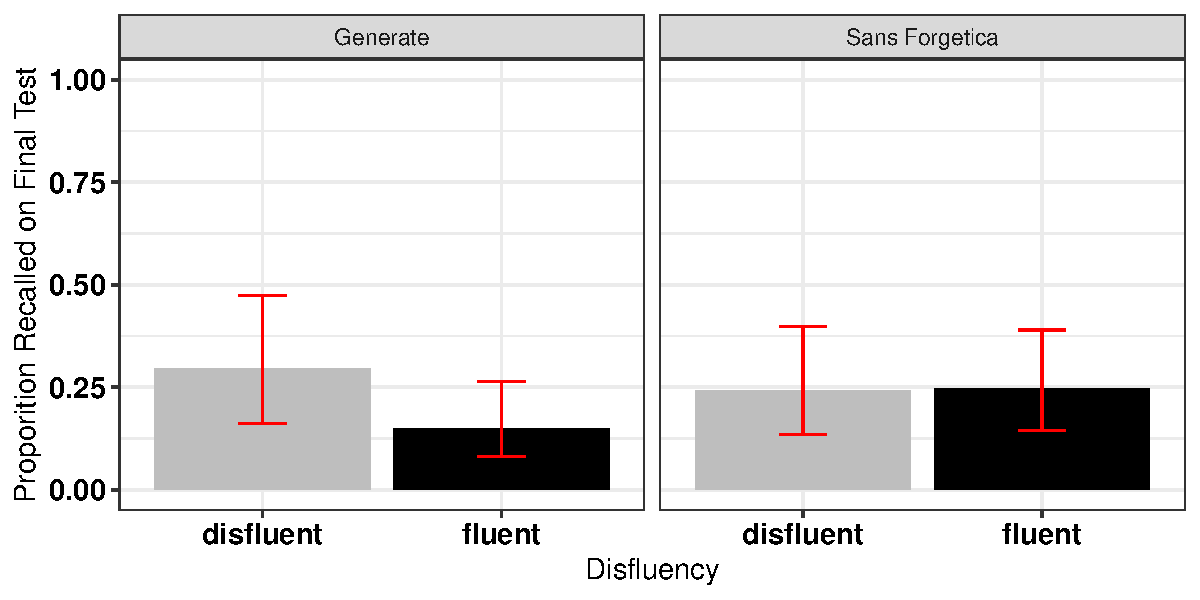
\includegraphics{SF_Paper_files/figure-latex/unnamed-chunk-2-1.pdf}

\hypertarget{exploratory}{%
\section{Exploratory}\label{exploratory}}

In Experiment 2 we also asked students about their metacognitive awarness. Specifically we asked them: \enquote{How likely is it that you will be able to recall material from the passage you just read on a scale of 0 (not likely to recall) to 100 (likely to recall) in 5 minutes?} Initials analyses suggest that the normal passage was given higher JOLs (\emph{M} = 57.4, \emph{SE} = 1.97) than the pre-highlighted passage (\emph{M} = 50.3, \emph{SE} = 1.97), t(525) = -7.08, \emph{p} = .023. There were no reliable differences between the pre-highlighted passage and Sans Forgetica (\emph{M} = 53.8, \emph{SE} = 1.97), \emph{t}(525) = -3.52, \emph{p} = .415 or between the passage in Sans Forgetica and the passage presneted normally, \emph{t}(525) = 3.56, \emph{p} = .406.

One potential reason for pre-highlighted information recieving lower JOLs than the normal passage is that pre-highlighted information served to focus participants attention specific parts of the passage. Given the question, pariticpants might thought this would hinder them if tested over the passage as a whole. Future research should

\begin{tabular}{l|r|r|r|r|r}
\hline
contrast & estimate & SE & df & t.ratio & p.value\\
\hline
Highlight - Normal & -7.079546 & 2.7792 & 525 & -2.547332 & 0.0299152\\
\hline
Highlight - Passage & -3.517046 & 2.7792 & 525 & -1.265488 & 0.4153929\\
\hline
Normal - Passage & 3.562500 & 2.7792 & 525 & 1.281844 & 0.4060534\\
\hline
\end{tabular}

\begin{verbatim}
## List of 14
##  $ text            :List of 11
##   ..$ family       : NULL
##   ..$ face         : NULL
##   ..$ colour       : NULL
##   ..$ size         : num 10
##   ..$ hjust        : NULL
##   ..$ vjust        : NULL
##   ..$ angle        : NULL
##   ..$ lineheight   : NULL
##   ..$ margin       : NULL
##   ..$ debug        : NULL
##   ..$ inherit.blank: logi FALSE
##   ..- attr(*, "class")= chr [1:2] "element_text" "element"
##  $ axis.title.x    :List of 11
##   ..$ family       : NULL
##   ..$ face         : NULL
##   ..$ colour       : NULL
##   ..$ size         : num 16
##   ..$ hjust        : NULL
##   ..$ vjust        : NULL
##   ..$ angle        : NULL
##   ..$ lineheight   : NULL
##   ..$ margin       : NULL
##   ..$ debug        : NULL
##   ..$ inherit.blank: logi FALSE
##   ..- attr(*, "class")= chr [1:2] "element_text" "element"
##  $ axis.title.y    :List of 11
##   ..$ family       : NULL
##   ..$ face         : NULL
##   ..$ colour       : NULL
##   ..$ size         : num 16
##   ..$ hjust        : NULL
##   ..$ vjust        : NULL
##   ..$ angle        : NULL
##   ..$ lineheight   : NULL
##   ..$ margin       : NULL
##   ..$ debug        : NULL
##   ..$ inherit.blank: logi FALSE
##   ..- attr(*, "class")= chr [1:2] "element_text" "element"
##  $ axis.text       :List of 11
##   ..$ family       : NULL
##   ..$ face         : NULL
##   ..$ colour       : NULL
##   ..$ size         : num 14
##   ..$ hjust        : NULL
##   ..$ vjust        : NULL
##   ..$ angle        : NULL
##   ..$ lineheight   : NULL
##   ..$ margin       : NULL
##   ..$ debug        : NULL
##   ..$ inherit.blank: logi FALSE
##   ..- attr(*, "class")= chr [1:2] "element_text" "element"
##  $ axis.text.x     :List of 11
##   ..$ family       : NULL
##   ..$ face         : NULL
##   ..$ colour       : NULL
##   ..$ size         : NULL
##   ..$ hjust        : NULL
##   ..$ vjust        : num 0.5
##   ..$ angle        : num 45
##   ..$ lineheight   : NULL
##   ..$ margin       : NULL
##   ..$ debug        : NULL
##   ..$ inherit.blank: logi FALSE
##   ..- attr(*, "class")= chr [1:2] "element_text" "element"
##  $ axis.line.x     :List of 6
##   ..$ colour       : chr "black"
##   ..$ size         : num 0.5
##   ..$ linetype     : chr "solid"
##   ..$ lineend      : NULL
##   ..$ arrow        : logi FALSE
##   ..$ inherit.blank: logi FALSE
##   ..- attr(*, "class")= chr [1:2] "element_line" "element"
##  $ axis.line.y     :List of 6
##   ..$ colour       : chr "black"
##   ..$ size         : num 0.5
##   ..$ linetype     : chr "solid"
##   ..$ lineend      : NULL
##   ..$ arrow        : logi FALSE
##   ..$ inherit.blank: logi FALSE
##   ..- attr(*, "class")= chr [1:2] "element_line" "element"
##  $ legend.text     :List of 11
##   ..$ family       : NULL
##   ..$ face         : NULL
##   ..$ colour       : NULL
##   ..$ size         : num 16
##   ..$ hjust        : NULL
##   ..$ vjust        : NULL
##   ..$ angle        : NULL
##   ..$ lineheight   : NULL
##   ..$ margin       : NULL
##   ..$ debug        : NULL
##   ..$ inherit.blank: logi FALSE
##   ..- attr(*, "class")= chr [1:2] "element_text" "element"
##  $ legend.title    :List of 11
##   ..$ family       : NULL
##   ..$ face         : NULL
##   ..$ colour       : NULL
##   ..$ size         : num 16
##   ..$ hjust        : NULL
##   ..$ vjust        : NULL
##   ..$ angle        : NULL
##   ..$ lineheight   : NULL
##   ..$ margin       : NULL
##   ..$ debug        : NULL
##   ..$ inherit.blank: logi FALSE
##   ..- attr(*, "class")= chr [1:2] "element_text" "element"
##  $ legend.position : chr "right"
##  $ panel.border    : list()
##   ..- attr(*, "class")= chr [1:2] "element_blank" "element"
##  $ panel.grid.major: list()
##   ..- attr(*, "class")= chr [1:2] "element_blank" "element"
##  $ panel.grid.minor: list()
##   ..- attr(*, "class")= chr [1:2] "element_blank" "element"
##  $ plot.title      :List of 11
##   ..$ family       : NULL
##   ..$ face         : chr "bold"
##   ..$ colour       : NULL
##   ..$ size         : num 16
##   ..$ hjust        : NULL
##   ..$ vjust        : NULL
##   ..$ angle        : NULL
##   ..$ lineheight   : num 0.8
##   ..$ margin       : NULL
##   ..$ debug        : NULL
##   ..$ inherit.blank: logi FALSE
##   ..- attr(*, "class")= chr [1:2] "element_text" "element"
##  - attr(*, "class")= chr [1:2] "theme" "gg"
##  - attr(*, "complete")= logi FALSE
##  - attr(*, "validate")= logi TRUE
\end{verbatim}

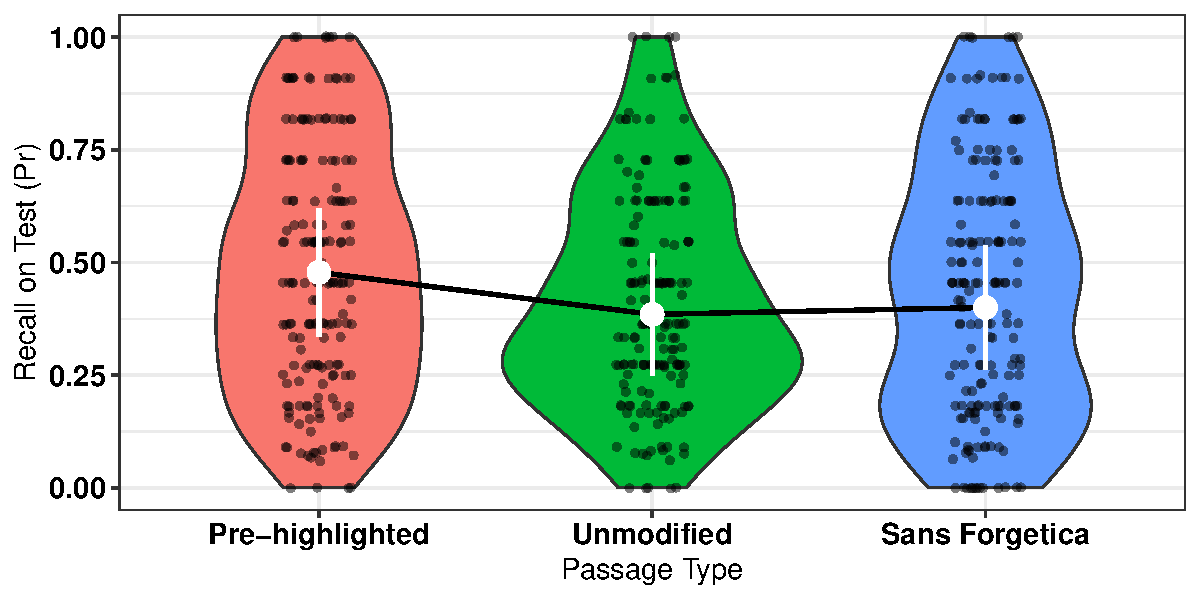
\includegraphics{SF_Paper_files/figure-latex/unnamed-chunk-3-1.pdf}

We hypothezied that sentences pre-highlighted or presented in sans forgetica would be better remembered than sentences presented normally. Further, we predicted that there would be no recall differences between the pre-highligted and the sans forgetica conditions. Our hypothese were only partially confirmed. We found that infromation that was pre-hightlighted had better recall than passages presentened normally, \emph{Estimate} = -.328, \emph{SE} = .166, \emph{z} = -1.97, \emph{p} = .048. Sentences that were pre-highlighted were also remembered marginally better than senetnces presented in sans forgetica,\emph{Estimate} = -.307, \emph{SE} = .167, \emph{z} = -1.84, \emph{p} = .066. Looking at Bayes Factor for this comparison suggests that evidence for a difference between the two conditions is faily weak. Critically, sentences presented in sans forgetcia were not better remembered than sentences presented normally, \emph{Estimate} = -.328, \emph{SE} = .166, \emph{z} = -1.97, \emph{p} = .048, \emph{BF}=).

\hypertarget{conclusions}{%
\section{Conclusions}\label{conclusions}}

The evidence contained herein suggests that SF does not have the mnemonic effects pruported by its creators. Now it is possible that there is an effect of SF, but the effect size might be smaller than we could detect acorss our two studies. Our SESOI was d = .35. If so, it probably does not have any real educational benefit. It is our conclsuion that SF is really forgetable and you should not be using it as a way to boost leanring.

\newpage

\hypertarget{references}{%
\section{References}\label{references}}

\begingroup
\setlength{\parindent}{-0.5in}
\setlength{\leftskip}{0.5in}

\hypertarget{refs}{}

\endgroup

\end{document}
